\documentclass[12pt]{article}
\title{
        {GFS Gemeinschaftskunde} \\
    {\large Was sind die Ursachen des Nichtwählens?}\\
}
\author{Daniel Meiborg}
\date{\today}

\usepackage{amsmath}
\usepackage{dirtytalk}
\usepackage{graphicx}
\graphicspath{{assets/}}
%\usepackage[a4paper, top=2cm, left=2cm, right=2cm, bottom=2.5cm]{geometry}


\begin{document}

    \maketitle
    \newpage

    \tableofcontents
    \newpage


    \section{Einleitung}


    \section{Definition Nichtwähler}
    \say{Nichtwähler sind Wahlberechtigte, die ihr Wahlrecht nicht in Anspruch nehmen, indem sie nicht zur Wahl gehen
    und auch nicht per Briefwahl wählen.}\cite{bundeswahlleiter2021nichtwaehler}


    \section{Wahlbeteiligung in Deutschland}


    \begin{figure}
        \centering
        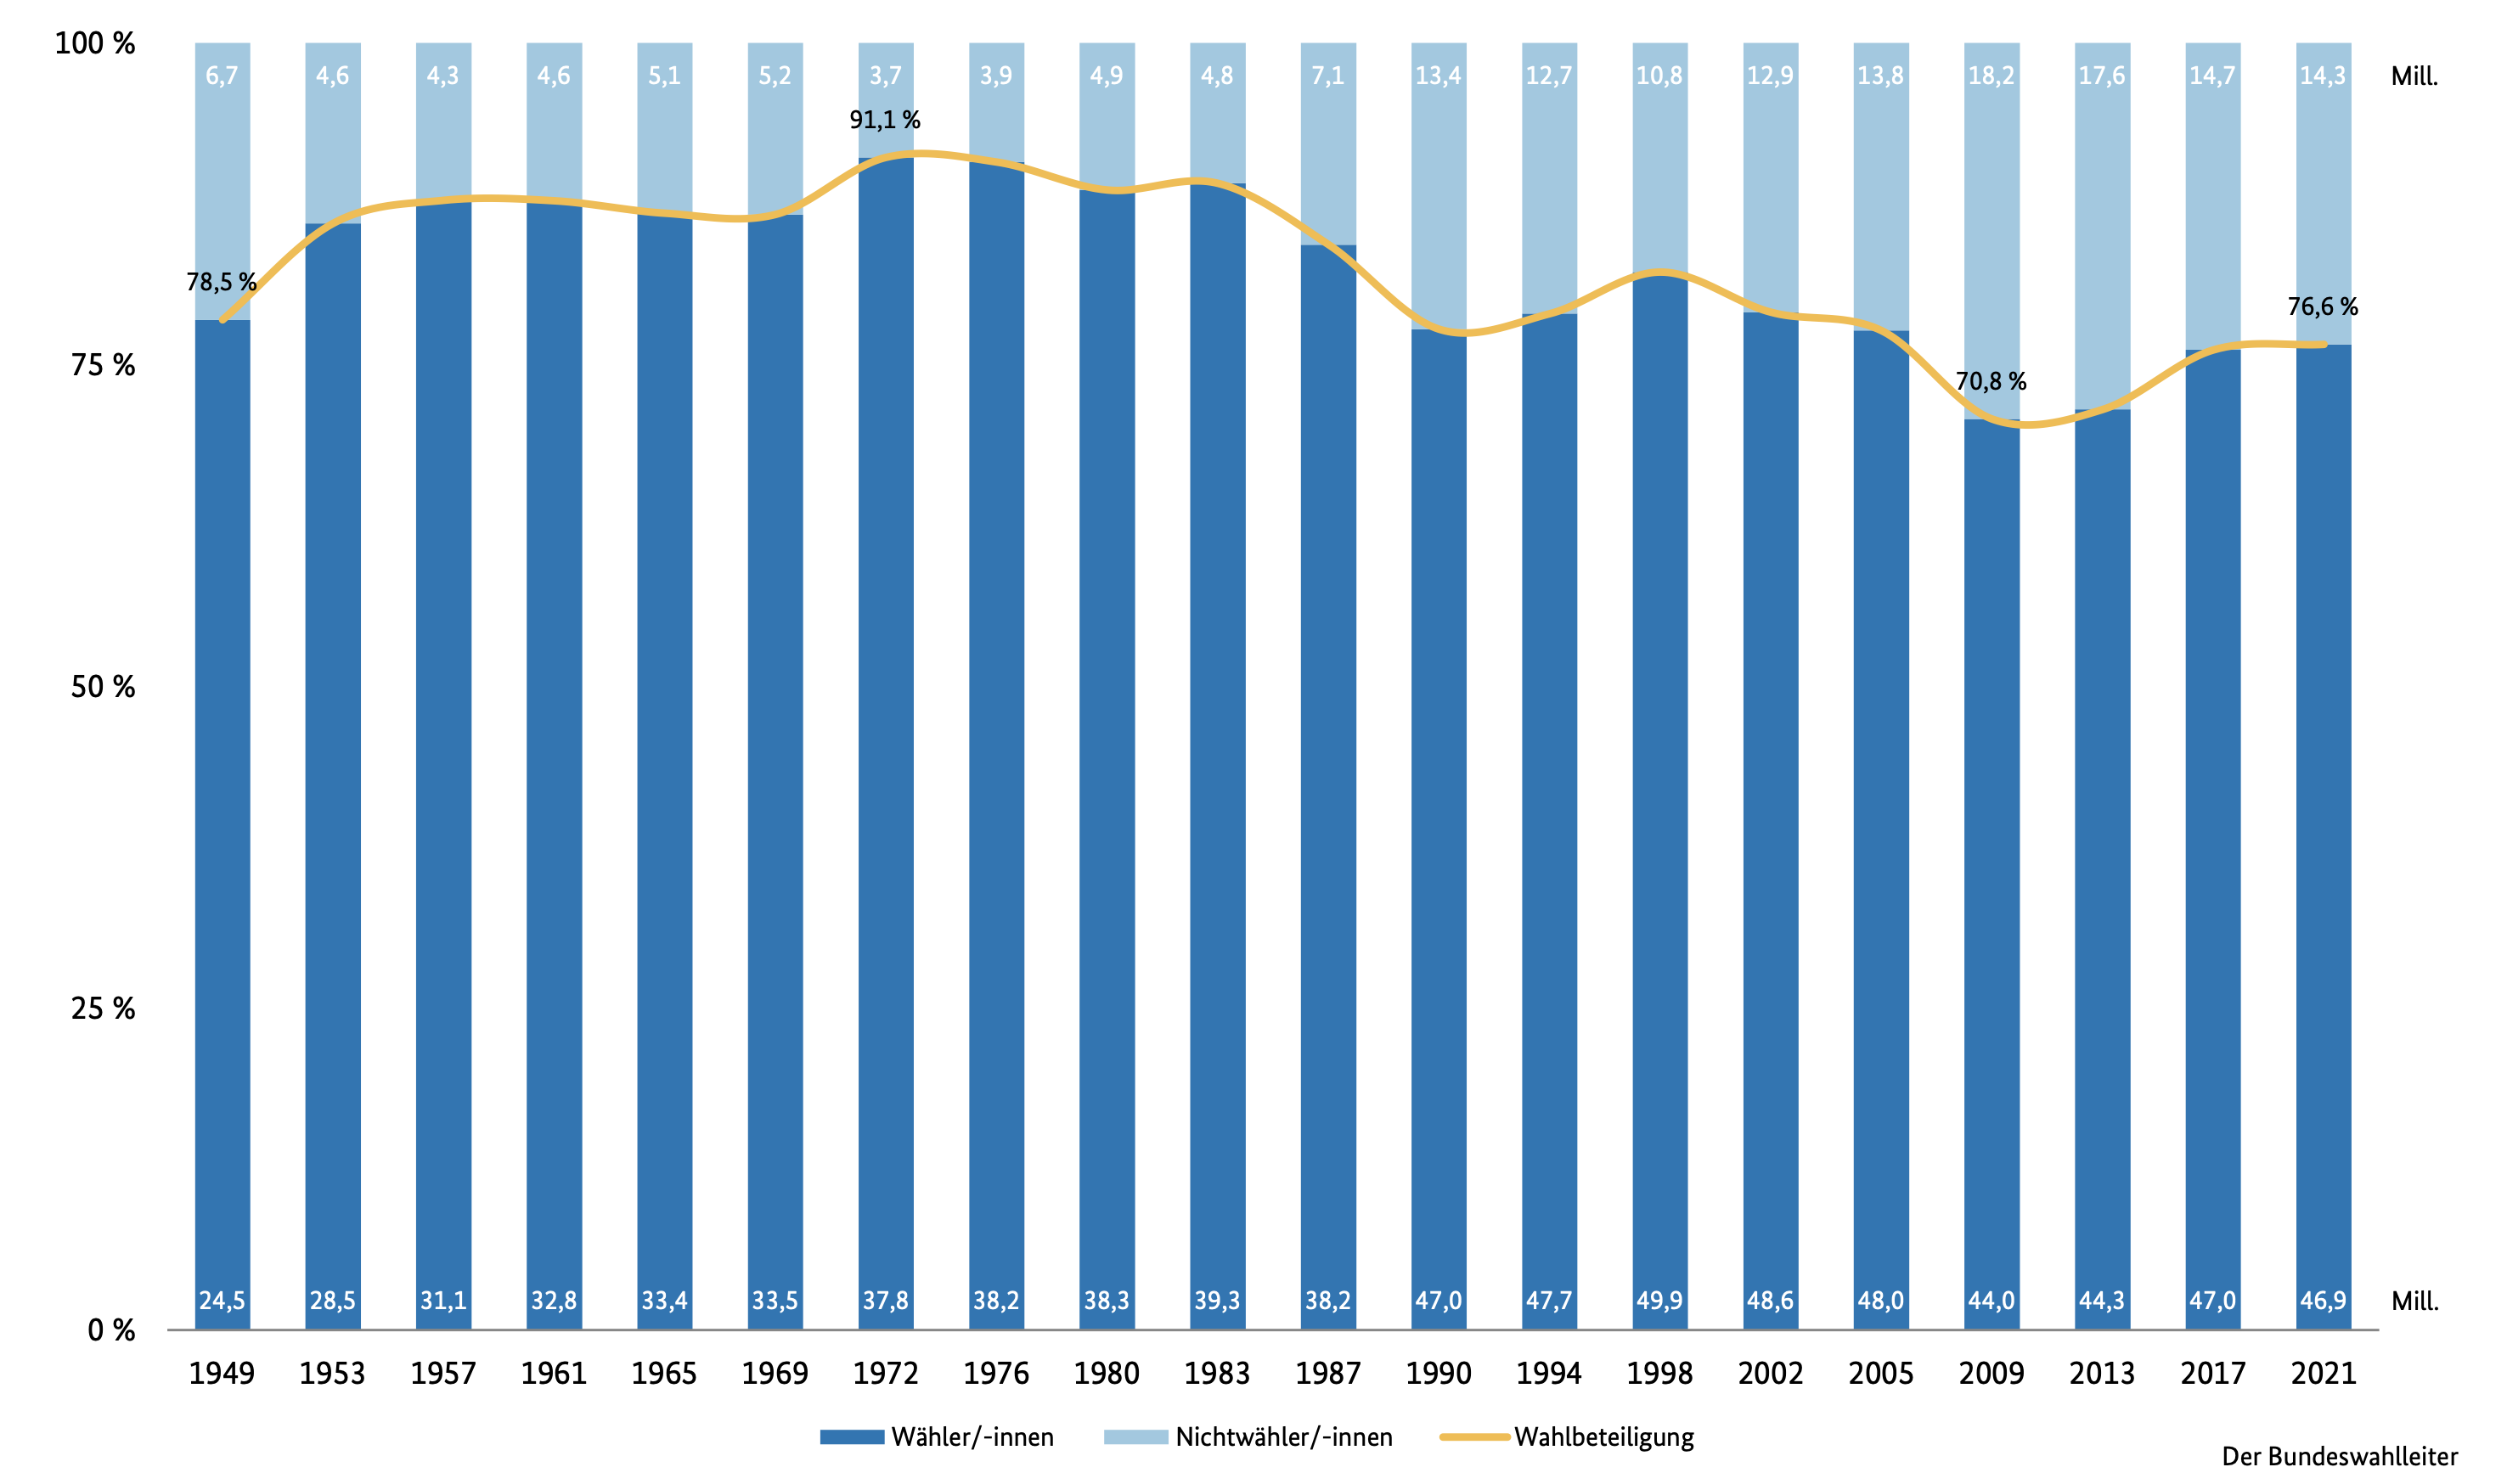
\includegraphics[width=\textwidth]{assets/Statistik-Wahlbeteiligung-Deutschland-seit-1949}
        \caption{Wahlbeteiligung in Deutschland seit 1949~\cite{bundeswahlleiter2021wahlbeteiligung}}
    \end{figure}


    \section{Ursachen des Nichtwählens}

    \subsection{Normalisierungsthese}

    \subsection{Krisenthese}

    \subsection{Probleme des Nichtwählens}


    \section{Lösung Wahlpflicht?}


    \section{Fazit}


    \section{Eigenständigkeitserklärung}

    \bibliography{main}
    \bibliographystyle{plain}

\end{document}